%\documentclass[12pt,a4paper]{report}
\documentclass[12pt,a4paper]{article}

\usepackage[brazil]{babel}
\usepackage[utf8]{inputenc}
\usepackage[T1]{fontenc}
\usepackage{graphicx,url}
\usepackage{hyperref}
%\usepackage{mathptmx}
\usepackage{lipsum}
\usepackage{booktabs}
\usepackage{pifont}
\usepackage{textcomp}
\usepackage{amsmath,amssymb}
\usepackage{listings}
\usepackage[scaled=0.8]{beramono}
\usepackage{xspace}
\usepackage{pdfpages}
\usepackage{listings}
\usepackage{xcolor}

\pdfgentounicode=1

\newcommand{\HRule}{\rule{\linewidth}{0.5mm}}

\lstdefinestyle{c}{%
    language=C,
    basicstyle=\ttfamily,
    numbers=left,
    breaklines=true,
    belowcaptionskip=1\baselineskip,
    aboveskip=1\baselineskip,
    belowskip=1\baselineskip,
    moredelim=**[is][\color{red}]{@}{@}
}

\lstset{%
    basicstyle=\ttfamily,
    aboveskip=1\baselineskip,
    belowskip=1\baselineskip,
    extendedchars=true,
    literate={á}{{\'a}}1 {ã}{{\~a}}1 {é}{{\'e}}1
}

\renewcommand{\lstlistingname}{Código}

\begin{document}

\begin{titlepage}

\begin{center}


\includegraphics[width=1.0\textwidth]{img/unb_logo.jpg}~\\[1cm]

\textsc{\Large Programação Paralela}\\[0.5cm]

% Title
\HRule\\[0.4cm]
{\huge \bfseries Relatório do Exercício 3\\[0.4cm]}
\HRule\\[1.5cm]

% Author and Supervisor
\begin{minipage}{0.4\textwidth}
\begin{flushleft} \large
\textit{Autor:}\\
\small{Alexandre Lucchesi Alencar}
\end{flushleft}
\end{minipage}
\begin{minipage}{0.4\textwidth}
\begin{flushright} \large
\textit{Professor:}\\
\small{George Luiz Medeiros Teodoro}
\end{flushright}
\end{minipage}

\vfill

% Bottom of the page
{\large \today}

\end{center}

\end{titlepage}



\section{Introdução}
Este relatório tem como objetivo apresentar os resultados obtidos a partir da
execução do terceiro exercício de programação paralela~\cite{exercise}, que
consiste na implementação de uma árvore de redução de soma (\textit{sum tree})
utilizando Message Passing Interface (MPI)~\footnote{Neste trabalho, utilizou-se
a implementação OpenMPI para Mac OS X, instalada a partir do utilitário
Homebrew.}. Primeiramente, os aspectos principais do algoritmo desenvolvidos são
apresentados. Em seguida, é realizada uma análise de desempenho comparando os
tempos de execução do algoritmo em diversas configurações, isto é, variando-se o
número de processos e a quantidade de números de ponto-flutuante a serem
somados. O código-fonte completo deste trabalho, incluindo os arquivos
\LaTeX\xspace que compõem este relatório, estão publicamente disponíveis no
GitHub~\footnote{\url{https://github.com/alexandrelucchesi/parallel-programming-ex03}}.

\subsection{\textit{Hardware} Utilizado}
\label{sec:hardware}

\begin{itemize}
    \item Processador: AMD FX(tm)-8350 Eight-Core Processor
    \item Velocidade por \textit{core}: 1406.2 MHz
    \item Número de processadores: 1
    \item Número de \textit{cores}: 8 (máx. 8)
    \item Número de \textit{threads}: 8 (máx. 8)
    \item L1 Data cache: 8 x 16 KBytes, 4-way set associative, 64-byte line size
    \item L1 Instruction cache: 4 x 64 KBytes, 2-way set associative, 64-byte line size
    \item L2 cache: 4 x 2048 KBytes, 16-way set associative, 64-byte line size
    \item L3 cache: 8 MBytes, 64-way set associative, 64-byte line size
\end{itemize}


\section{O Algoritmo}


\subsection{Artefatos Desenvolvidos}
O programa desenvolvido possui duas funcionalidades principais: (i) geração de
um arquivo de dados contendo um número arbitrário de valores de ponto-flutuante;
(ii) e processamento de um arquivo de dados retornando a soma dos elementos e o
tempo de execução do algoritmo. Além do programa principal, foram desenvolvidos
dois \textit{scripts bash}: um para facilitar a execução do programa principal,
encapsulando a chamada ao \texttt{mpiexec} (ou \texttt{mpirun}), e outro para
automatizar os testes da aplicação. Esses artefatos são descritos a seguir.

\begin{itemize}
    \item \texttt{main.c}: programa em C contendo o código-fonte da aplicação.
        Após compilado com o \texttt{mpicc} (vide Makefile), pode ser executado
        chamando-se o \textit{script} \texttt{run.sh} passando-se o número de
        processos e o arquivo de dados. O \texttt{run.sh} executará o programa
        usando o \texttt{mpiexec} e passando esses dois argumentos, que são
        recebidos via \texttt{scanf()}. A saída do programa é uma linha contendo
        dois números: o primeiro representa o resultado da soma dos números de
        ponto-flutuante e o segundo, o tempo de execução do algoritmo de redução
        em milisegundos (desconsiderando o tempo de entrada de dados).
	\item \texttt{test.sh}: \textit{script} desenvolvido para automatizar os
		testes da aplicação. Recebe como entrada 2 argumentos, em ordem:
		\begin{itemize}
			\item \texttt{max\_numbers}: número máximo de processos. O
				\textit{script} varia o número de processos de $2^{20}$ até
				$2^{max\_numbers}$.
			\item \texttt{max\_runs}: número máximo de vezes em que o programa
				deve ser executado em uma mesma configuração.
		\end{itemize}
\end{itemize}


\subsection{Geração do Arquivo de Dados}
\label{sec:data-gen}
Para a geração de quantidades configuráveis de números de ponto-flutante em um
formato apropriado para servir de entrada para o programa, pode-se executar o
binário proveniente do processo de compilação diretamente. Por exemplo, para
gerar um arquivo de dados, \texttt{numbers.dat}, contendo, por exemplo, 64
elementos, basta executar o binário passando-se a \textit{flag} \texttt{-gen},
conforme descrito a seguir:

\begin{lstlisting}[language=bash]
$ make      # Gera o binário com nome: 'sumtree'.
$ ./sumtree -gen numbers.dat 64
\end{lstlisting}

Uma outra opção disponível é a \texttt{-{}-help}, que exibe informações de uso da
aplicação.


\subsection{Função de ``Espalhamento''}
Para distribuir os dados entre os diferentes processos, foram criadas duas
funções:

\begin{lstlisting}[style=c, numbers=none]
void scather(int my_rank, int comm_sz,
    unsigned int *my_count, float **my_nums);
void scather_intercalate(int my_rank, int comm_sz,
    unsigned int *my_count, float **my_nums);
\end{lstlisting}

Uma sempre pode ser utilizada no lugar da outra sem alterar o resultado final
(note que a assinatura é a mesma). A única diferença está na política de
atribuição dos números aos processos. Internamente, o processo com
\texttt{my\_rank} igual a zero é sempre o responsável por ler o arquivo de dados
e dividir os números entre os \texttt{comm\_sz} processos, retornando em
\texttt{my\_count} e \texttt{my\_nums} a quantidade de elementos e os números,
respectivamente.

No caso da \texttt{scather}, a quantidade total de números (lida do arquivo de
entrada) é dividida pelo número de processos (\texttt{comm\_sz}) e o resultado
(\texttt{res}) obtido é utilizado para atribuir sequencialmente os números aos
processos, ou seja, o processo 0 recebe os números indexados pelo intervalo $[0,
res - 1]$, o processo 1 recebe $[res, 2 \times res - 1]$, e assim por diante.

Por outro lado, a \texttt{scather\_intercalate} intercala os números entre os
processos, varrendo o vetor e atribuindo o elemento no índice $i$ ao processo $i
\bmod comm\_sz$. 


\subsection{Evitando \textit{Deadlocks}}
Na implementação do MPI utilizada, ambas as primitivas \texttt{Send()} e
\texttt{Recv()} são ``blocantes''. Isso significa que cuidado adicional deve ser
tomado para que não ocorram \textit{deadlocks}. O trecho de
código~\ref{code:deadlock} apresenta como a função \texttt{reduce\_sumtree()}
foi projetada para evitar a ocorrência de \textit{deadlocks}.

\begin{minipage}{\linewidth}
\begin{lstlisting}[frame=single, style=c, label={code:deadlock},
    caption={Ordem das primitivas MPI\_Send() e MPI\_Recv() na função \texttt{reduce\_sumtree()}.}]
...
if (my_rank % 2 == 0) {
    int dst = my_rank + 1;

    // Copy second half of `nums[]` to `my_nums`.
    memcpy(my_nums, nums + qty, qty * sizeof(float));

    // Send first half of `nums[]` to `dst`.
    @MPI_Send(nums, qty, MPI_FLOAT, dst, 2, MPI_COMM_WORLD);@

    // Receive second half of his `nums[]` into `his_nums`.
    @MPI_Recv(his_nums, qty, MPI_FLOAT, dst, 2, MPI_COMM_WORLD, MPI_STATUS_IGNORE);@
} else {
    int dst = my_rank - 1;

    // Copy first half of `nums[]` to `my_nums`.
    memcpy(my_nums, nums, qty * sizeof(float));

    // Receive first half of his `nums[]` into `his_nums`.
    @MPI_Recv(his_nums, qty, MPI_FLOAT, dst, 2, MPI_COMM_WORLD, MPI_STATUS_IGNORE);@

    // Send second half of `nums[]` to `dst`.
    @MPI_Send(nums + qty, qty, MPI_FLOAT, dst, 2, MPI_COMM_WORLD);@
}
...
\end{lstlisting}
\end{minipage}

Se as primitivas \texttt{MPI\_Recv()} e \texttt{MPI\_Send()} aparecerem na mesma
ordem no \texttt{if} e no \texttt{else}, os processos entrarão em
\textit{deadlock}. Ao colocá-los de forma alternada, garante-se que para cada
\texttt{MPI\_Send()} existirá um \texttt{MPI\_Recv()} e vice-versa.

\section{Medida de Tempo de Execução}
Para medir o tempo máximo de execução da aplicação de forma precisa, utilizou-se
\emph{barreiras}. Com uma chamada à função \texttt{MPI\_Barrier()} antes de
\texttt{reduce\_sumtree()}, garante-se que todos os processos começam a executar
o algoritmo de redução ``ao mesmo tempo''. Com outra chamada à função
\texttt{MPI\_Barrier()} após a chamada à \texttt{reduce\_sumtree()} é possível
sincronizar todos os processos no ponto de término da execução do algoritmo.
Dessa forma, coletando os tempos (``relógio de parede'') no processo 0
imediatamente após as barreiras, é possível calcular o tempo total de execução
da aplicação.

Utilizou-se a função \texttt{gettimeofday()} (disponível em
``\texttt{sys/time.h}'') para se obter os tempos de início e término e
aritmética simples para se obter o intervalo de execução em milisegundos.

\section{Resultados}
\label{sec:resultados}
Executou-se o \textit{script} de testes (\texttt{test.sh}) passando-se como
argumentos: 25 \texttt{max\_numbers}, para executar testes variando-se a
quantidade de elementos de $2^{20}$ à $2^{25}$; e 5 \texttt{max\_runs}, para se
realizar 5 execuções em cada configuração.

O \textit{script} \texttt{test.sh} gerou como saída arquivos de dados contendo
os números de ponto-flutuante para serem usados nos testes (extensão
\texttt{.dat}) e arquivos no formato CSV contendo as tabelas que compõem este
relatório. Cada tabela é indexada pela quantidade de elementos (no exemplo
acima, de $10^{20}$ à $10^{25}$) e o número da execução (no exemplo acima, de 1
a 5). Metade possui o prefixo \texttt{sum\_{n}}, onde \texttt{n} é o número de
processos utilizado, representando os valores aproximados da soma calculados. A
outra metade possui prefixo \texttt{time\_{n}}, e contém os valores dos tempos
de execução.  Em poucas palavras, tem-se 2 arquivos para cada número de
processos contendo as duas saídas do programa: o valor estimado da soma e o
tempo de execução do algoritmo.

As seções a seguir apresentam os resultados dos testes, apresentando métricas de
\textit{speedup}, eficiência e escalabilidade. Os resultados são apresentados
sob a forma de gráficos. As tabelas com os dados exatos que deram origem a esses
gráficos estão anexadas ao final do documento.

\subsection{\textit{Speedup}}
\begin{figure}[h!]
\centering
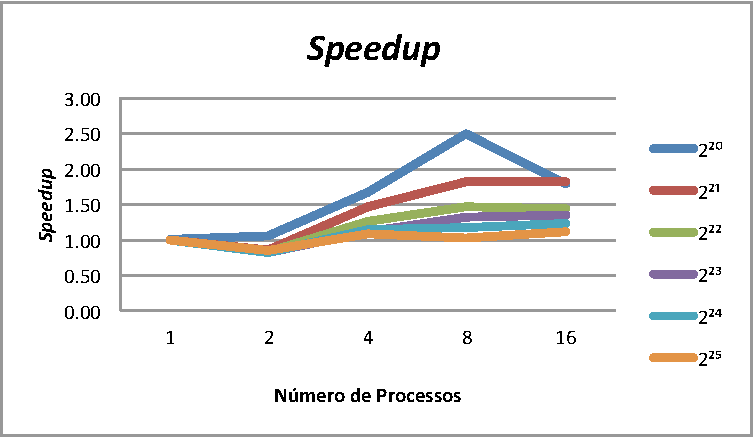
\includegraphics{img/speedup.pdf}
\caption{Gráfico apresentando a relação entre o \textit{speedup}, o número de
processos e a quantidade de elementos somados na redução.}
\label{fig:speedup}
\end{figure}

A Figura~\ref{fig:speedup} apresenta um gráfico em que cada curva relaciona o
\textit{speedup} obtido, o número de processos criados e a quantidade de
elementos somados na redução. De uma forma geral, observa-se que o
\textit{speedup} \emph{aumenta} conforme a quantidade de processos cresce. A
excessão ocorre apenas quando se utiliza dois processos, onde perde-se
desempenho para quase todos os tamanhos de entrada~\footnote{Com $2^{20}$
elementos houve um ganho de desempenho mínimo, com o \textit{speedup} no valor
de 1.04.}.

Isso ocorre porque o \textit{overhead} envolvido na criação de dois processos e,
principalmente, na comunicação entre os processos é maior do que os possíveis
ganhos advindos da concorrência entre os mesmos.

\subsection{Eficiência}

\begin{figure}[h!]
\centering
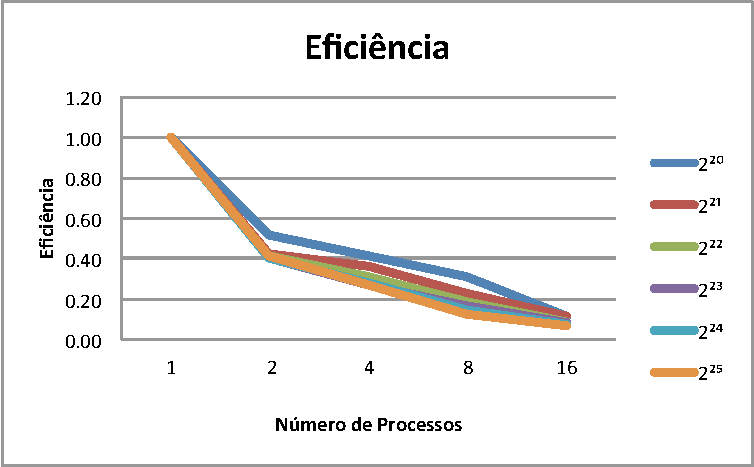
\includegraphics{img/efficiency.pdf}
\caption{Gráfico apresentando a relação entre o \textit{speedup}, o número de
processos e a quantidade de elementos somados na redução.}
\label{fig:efficiency}
\end{figure}

A Figura~\ref{fig:efficiency} apresenta um gráfico em que cada curva relaciona a
\textit{eficiência} obtida, o número de processos criados e a quantidade de
elementos somados na redução. De uma forma geral, observa-se que a
\textit{eficiência} \emph{diminui} conforme a quantidade de processos cresce.

\subsection{Escalabilidade}

Conforme ilustrado na Figura~\ref{fig:efficiency} e observando as tabelas de
tempo de execução ao final deste documento, nota-se que a eficiência cai em uma
taxa muito maior que os tempos de execução. Dessa forma, conclui-se que a
aplicação não possui uma boa \emph{escalabilidade forte}.

De forma similar, não se tem também uma boa \emph{escalabilidade fraca},
conforme apresentado na Figura~\ref{fig:weak-scalability}, que relaciona a
eficiência, o número de processos, e a quantidade de elementos somados na
redução. Não está explícito no gráfico, mas para cada número de processos
obteve-se o valor da eficiência de acordo incrementando-se proporcionalmente o
tamanho do problema (ou número de elementos a serem somados). Sendo assim, para
1 processo, utilizou-se $2^20$ elementos; para 2 processos, $2^21$ elementos;
para 4 processos, $2^22$ elementos; e assim por diante.

\begin{figure}[h!]
\centering
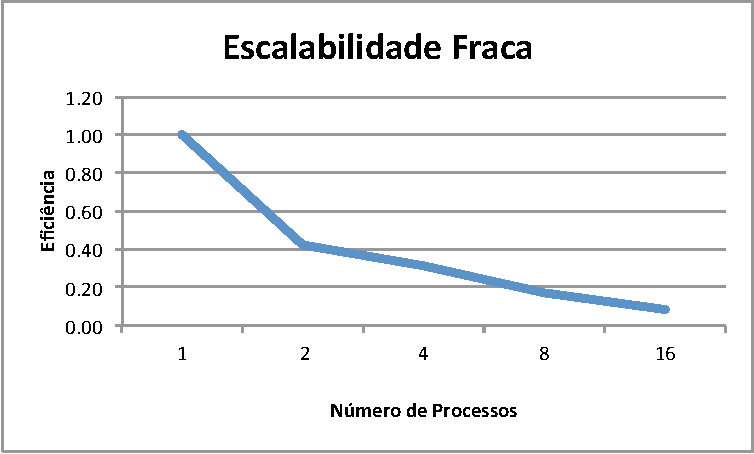
\includegraphics{img/weak-scalability.pdf}
\caption{Gráfico apresentando a relação entre a eficiência e o número de
processos, aumentando-se proporcionalmente o tamanho do problema.}
\label{fig:weak-scalability}
\end{figure}


\section{Conclusão}
Este trabalho possibilitou uma maior compreensão acerca de modelos de
programação baseados em trocas de mensagem, em particular, que utilizam
primitivas \texttt{Send()} e \texttt{Recv()}, através da implementação de uma
árvore de redução de soma usando MPI\@.

O algoritmo desenvolvido possibilita a simulação de reduções usando um número
grande de processos, utilizando as primitivas citadas anteriormente para
realizar somas intermediárias até chegar na redução a partir de uma \emph{Sum
Tree}. Uma análise dos tempos de execução do algoritmo evidenciou ganhos de
desempenho (\textit{speedup}) de até 252\% em relação à versão sequencial.

Por fim, é válido ressaltar que o o \textit{design} da aplicação (incluindo o
\textit{script} \texttt{test.sh}) permite variar de forma fácil as condições de
teste, permitindo a reprodução dos experimentos apresentados neste trabalho e
facilitando a experimentação com novas configurações. 

\bibliographystyle{plain}
\bibliography{references.bib}


% ANEXO
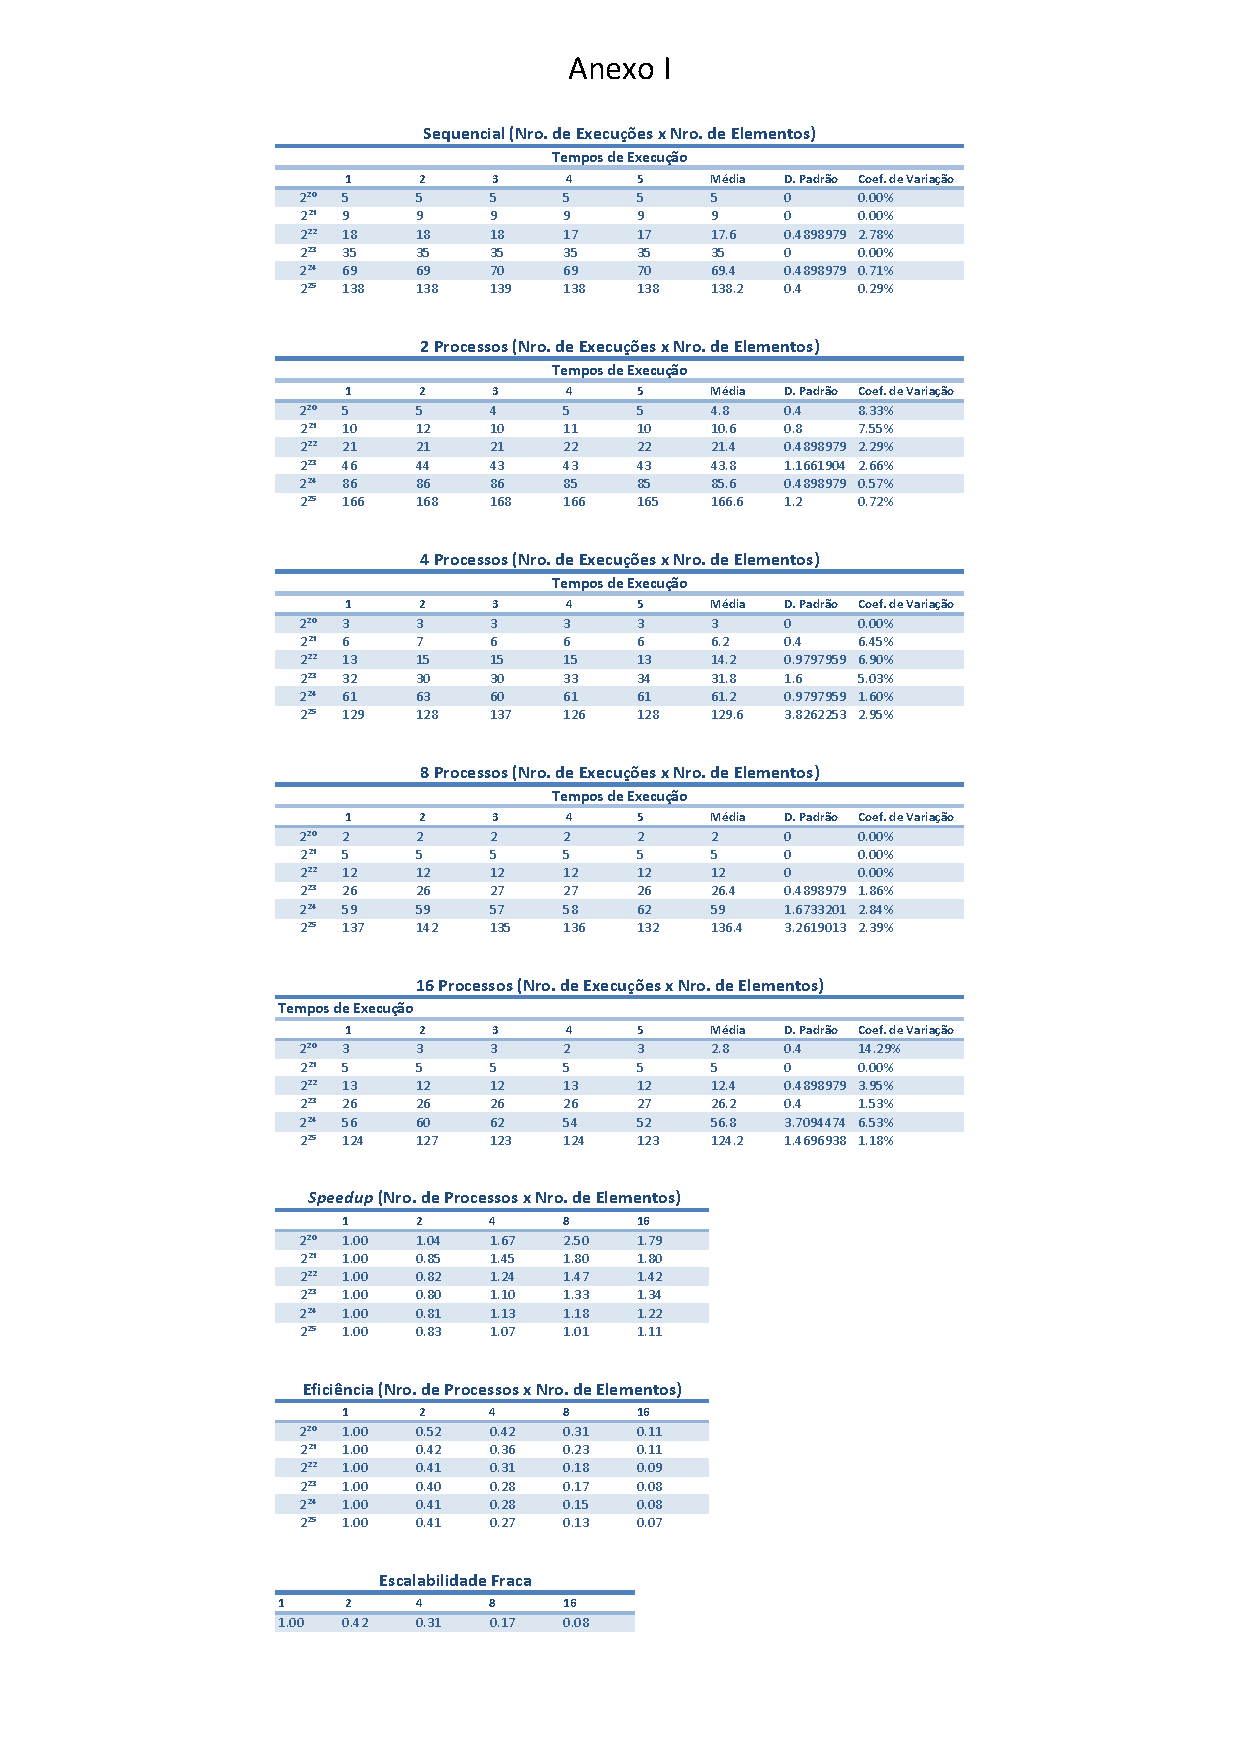
\includepdf[pages={1-},scale=1.0,landscape=false]{./img/bench-tables.pdf}


\end{document}








